\documentclass[aspectratio=169,11pt]{beamer}

\usepackage{plex-serif}
\renewcommand{\familydefault}{\rmdefault}
\usepackage[T1]{fontenc}
\usepackage{amsmath,amssymb,bm}
\usepackage{pifont}
\usepackage{tikz}
\usepackage{etoolbox}
\usetikzlibrary{
  calc,
  positioning,
  shapes.geometric,
  arrows.meta,
  overlay-beamer-styles
}

% ---------- Your Theme Palette ----------
\definecolor{navy}{HTML}{002B55}
\definecolor{steel}{HTML}{4D6FAD}
\definecolor{sky}{HTML}{5DADF5}
\definecolor{teal}{HTML}{3F8C8A}
\definecolor{slate}{HTML}{5B6475}
\definecolor{paper}{HTML}{FBFAF7}
\definecolor{ink}{HTML}{1C2233}
\colorlet{deepteal}{navy!55!teal}

% ---------- Beamer Theme ----------
\setbeamercolor{background canvas}{bg=paper}
\setbeamercolor{normal text}{fg=ink}
\setbeamercolor{alerted text}{fg=teal}
\setbeamercolor{structure}{fg=navy}
\setbeamertemplate{navigation symbols}{}

\setbeamertemplate{background}{
  \begin{tikzpicture}[remember picture,overlay,shift={(current page.south west)}]
    \clip (0,0) rectangle (16,9);
  \end{tikzpicture}
}

\setbeamertemplate{frametitle}{%
  \begin{tikzpicture}[remember picture,overlay,shift={(current page.north west)}]
    \fill[navy] (0,0) rectangle (16,-1.05);
   
    \node[anchor=west,text=white,font=\fontseries{eb}\selectfont\Large] at (0.72,-0.525)
      {\insertframetitle};
  \end{tikzpicture}
  \vspace*{0.78cm}}

\setbeamertemplate{footline}{%
  \begin{tikzpicture}[remember picture,overlay,shift={(current page.south west)}]
    \node[anchor=west,font=\scriptsize,text=steel] at (0.72,0.32)
      {Variational Autoencoder \;\textcolor{slate!60}{|}\; CSE200};
    \node[anchor=east,font=\scriptsize\bfseries,text=steel] at (15.3,0.32)
      {\insertframenumber/\inserttotalframenumber};
  \end{tikzpicture}}

% ---------- Helpers ----------
\newenvironment{canvas}
  {\begin{tikzpicture}[remember picture,overlay,shift={(current page.south west)}]}
  {\end{tikzpicture}}

\tikzset{
  >={Stealth[length=2mm]},
  fwd/.style={->,line width=0.8pt,draw=ink},
  bigarrow/.style={fill=teal!35,draw=teal!80!black,line width=0.8pt},
  outline/.style={draw=teal,line width=1.55pt,fill=teal!8,opacity=0.18},
  box/.style={draw=navy,line width=1.25pt,rounded corners=5pt,fill=navy!4},
  hlt/.style={draw=teal,line width=1.55pt,fill=teal!8,opacity=0.18}
}


% ---------- Senior-style VAE diagram in your theme ----------
% Argument: input / encoder / latent / decoder / output / none
% Argument: input / encoder / latent / decoder / output / none

\newcommand{\VAEDiagram}[1]{

\begin{scope}[shift={(0.65,4.72)},scale=0.96]

  % =========================================================
  % INPUT x
  % =========================================================
  \fill[steel!18] (0.25,-1.00) rectangle (0.72,1.00);
  \draw[navy,line width=0.9pt] (0.25,-1.00) rectangle (0.72,1.00);
  \node[font=\scriptsize,text=navy] at (0.485,0) {$x$};

  % input -> encoder
  \draw[fwd] (0.72,0) -- (1.12,0);


  % =========================================================
  % ENCODER
  % =========================================================
  \node[
    trapezium,
    trapezium stretches=true,
    shape border rotate=270,
    minimum width=2.05cm,
    minimum height=1.65cm,
    draw=steel,
    line width=0.9pt,
    fill=steel!18,
    text=navy,
    font=\scriptsize
  ] (enc) at (1.95,0) {$h_{\phi}(x)$};


  % =========================================================
  % MU / LOG VARIANCE BRANCH
  % =========================================================

  \node[
    rectangle,
    minimum width=0.52cm,
    minimum height=0.78cm,
    draw=navy,
    line width=0.8pt,
    fill=navy!15,
    text=navy,
    font=\scriptsize
  ] (mu) at (3.6,0.68) {$\mu$};

  \node[
    rectangle,
    minimum width=0.6cm,
    minimum height=0.78cm,
    draw=steel,
    line width=0.8pt,
    fill=steel!18,
    text=navy,
    font=\tiny
  ] (logv) at (3.73,-0.68) {$\log\sigma^2$};

  % clean branch point
  \coordinate (branch) at (3.02,0);

  % =========================================================
% CLEAN ENCODER BRANCH
% =========================================================

% junction just after encoder
\coordinate (branch) at ($(enc.east)+(0.18,0)$);

% encoder -> junction
% no arrowhead here
\draw[ink,line width=0.8pt]
  (enc.east) -- (branch);

% vertical split
\draw[ink,line width=0.8pt]
  (branch) -- ($(branch)+(0,0.68)$);

\draw[ink,line width=0.8pt]
  (branch) -- ($(branch)+(0,-0.68)$);

% upper branch -> mu
% arrow points RIGHT into mu
\draw[fwd]
  ($(branch)+(0,0.68)$) -- (mu.west);

% lower branch -> log variance
% arrow points RIGHT into log sigma^2
\draw[fwd]
  ($(branch)+(0,-0.68)$) -- (logv.west);

  % =========================================================
  % BIG ARROW 1
  % =========================================================
  \draw[bigarrow]
  (4.28,-0.34) --
  (4.78,-0.34) --
  (4.78,-0.60) --
  (5.30,0) --
  (4.78,0.60) --
  (4.78,0.34) --
  (4.28,0.34) -- cycle;


  % =========================================================
  % LATENT DISTRIBUTION
  % =========================================================
  \node[font=\scriptsize,text=slate]
    at (5.64,0)
    {$\mathcal{N}($};

  \node[
    rectangle,
    minimum width=0.48cm,
    minimum height=0.70cm,
    draw=navy,
    fill=navy!15,
    text=navy,
    font=\scriptsize
  ] at (6.20,0) {$\mu$};

  \node[font=\scriptsize,text=slate]
    at (6.56,0)
    {$,$};

  \node[
    rectangle,
    minimum width=1.12cm,
    minimum height=0.70cm,
    draw=sky!80!navy,
    fill=sky!28,
    text=navy,
    font=\tiny
  ] at (7.20,0) {$\mathrm{diag}(\sigma^2)$};

  \node[font=\scriptsize,text=slate]
    at (7.96,0)
    {$)\sim$};


  % =========================================================
  % z
  % =========================================================
  \node[
    rectangle,
    minimum width=0.48cm,
    minimum height=0.78cm,
    draw=teal,
    fill=teal!22,
    text=navy,
    font=\scriptsize
  ] (z) at (8.47,0) {$z$};

  % z -> decoder
  \draw[fwd] (z.east) -- (9.02,0);


  % =========================================================
  % DECODER
  % =========================================================
  \node[
    trapezium,
    trapezium stretches=true,
    shape border rotate=90,
    minimum width=2.05cm,
    minimum height=1.65cm,
    draw=teal,
    line width=0.9pt,
    fill=teal!18,
    text=navy,
    font=\scriptsize
  ] (dec) at (9.9,0) {$f_{\theta}(z)$};

  % decoder -> psi
  \draw[fwd] (dec.east) -- (11.05,0);


  % =========================================================
  % psi
  % =========================================================
  \node[
    rectangle,
    minimum width=0.50cm,
    minimum height=1.20cm,
    draw=teal,
    fill=teal!18,
    text=navy,
    font=\scriptsize
  ] (psi) at (11.32,0) {$\psi$};


  % =========================================================
  % BIG ARROW 2
  % =========================================================
  \draw[bigarrow]
    (11.88,-0.34) --
    (12.38,-0.34) --
    (12.38,-0.60) --
    (12.90,0) --
    (12.38,0.60) --
    (12.38,0.34) --
    (11.88,0.34) -- cycle;


  % =========================================================
  % OUTPUT DISTRIBUTION
  % =========================================================
  \node[font=\scriptsize,text=slate]
    at (13.28,0)
    {$D($};

  \node[
    rectangle,
    minimum width=0.50cm,
    minimum height=1.20cm,
    draw=teal,
    fill=teal!18,
    text=navy,
    font=\scriptsize
  ] at (13.70,0) {$\psi$};

  \node[font=\scriptsize,text=slate]
    at (14.08,0)
    {$)\sim$};


  % =========================================================
  % OUTPUT x'
  % =========================================================
  \fill[steel!18] (14.45,-1.00) rectangle (14.92,1.00);
  \draw[navy,line width=0.9pt] (14.45,-1.00) rectangle (14.92,1.00);

  \node[font=\scriptsize,text=navy]
    at (14.685,0)
    {$x'$};


  % =========================================================
  % HIGHLIGHTS
  % =========================================================

  % INPUT
  \ifstrequal{#1}{input}{
    \draw[
      teal,
      line width=1.8pt,
      rounded corners=2pt
    ]
    (0.05,-1.18) rectangle (0.92,1.18);
  }{}


  % ENCODER
  \ifstrequal{#1}{encoder}{
    \draw[
      teal,
      line width=1.8pt,
      rounded corners=2pt
    ]
    (1.04,-1.30) rectangle (4.21,1.30);
  }{}


  % LATENT
  \ifstrequal{#1}{latent}{
    \draw[
      teal,
      line width=1.8pt,
      rounded corners=2pt
    ]
    (5.36,-1.28) rectangle (8.78,1.28);
  }{}


  % DECODER
  \ifstrequal{#1}{decoder}{
    \draw[
      teal,
      line width=1.8pt,
      rounded corners=2pt
    ]
    (8.96,-1.30) rectangle (11.72,1.30);
  }{}


  % OUTPUT
  \ifstrequal{#1}{output}{
    \draw[
      teal,
      line width=1.8pt,
      rounded corners=2pt
    ]
    (14.28,-1.18) rectangle (15.08,1.18);
  }{}

\end{scope}

}
% ---------- Text box ----------
\newcommand{\TextBox}[1]{
  \fill[navy!4,rounded corners=5pt] (0.78,1.35) rectangle (15.22,2.50);
  \draw[navy,line width=1.25pt,rounded corners=5pt] (0.78,1.35) rectangle (15.22,2.50);
  \node[anchor=west,text width=13.6cm,align=left,font=\footnotesize,text=ink]
    at (1.25,1.92) {#1};
}
\newcommand{\LatentNoteBox}[2]{%
  \fill[navy!4,rounded corners=5pt] (#1,1.05) rectangle (15.00,#2);
  \draw[navy,line width=1.25pt,rounded corners=5pt] (#1,1.05) rectangle (15.00,#2);
}


\title{Variational Autoencoder}

\begin{document}
% ================================================================
% INTRO SLIDE — BACK TO THE 80s
% ================================================================

\begin{frame}{Back to the 80's}
\begin{canvas}

% ------------------------------------------------
% Main image
% ------------------------------------------------
\node[
  anchor=center
] at (8.00,4)
{
  
\includegraphics[
    width=14.4cm,
    height=6.65cm,
    keepaspectratio
  ]{back_to_the_80.png}
};

\end{canvas}
\end{frame}

% =================================================================
% Slide 1: Input
% =================================================================
\begin{frame}{Input}
\begin{canvas}
  \VAEDiagram{input}
  \only<2->{\TextBox{The \textbf{Variational Autoencoder} begins with an input sample $x$, which can be an \textbf{image, text, or any data}.}}
\end{canvas}
\end{frame}

% =================================================================
% Slide 2: Encoder
% =================================================================
\begin{frame}{Encoder}
\begin{canvas}
  \VAEDiagram{encoder}
  \only<2->{
    \fill[navy!4,rounded corners=5pt] (0.78,1.05) rectangle (15.22,2.70);
    \draw[navy,line width=1.25pt,rounded corners=5pt] (0.78,1.05) rectangle (15.22,2.70);
    \node[anchor=west,text width=13.5cm,align=left,font=\footnotesize,text=ink] at (1.25,2.28)
      {$\bullet$ \; The \textbf{Encoder} maps the input $x$ into a \textbf{Latent Space Representation}.};
    \node[anchor=west,text width=13.5cm,align=left,font=\footnotesize,text=ink] at (1.25,1.82)
      {$\bullet$ \; Outputs:};
    \node[anchor=west,text width=13.5cm,align=left,font=\footnotesize,text=ink] at (1.75,1.42)
      {$\bullet$ \; \textbf{Mean} $(\mu)$ \qquad $\bullet$ \; \textbf{Log Variance} $(\log\sigma^2)$};
  }
\end{canvas}
\end{frame}

% =================================================================
% Slide 3: Latent Variable
\begin{frame}{Latent Variable}

\begin{canvas}

\begin{scope}[yshift=0.30cm]

  \VAEDiagram{latent}

  % First explanation box
  \only<1->{
    \fill[navy!4,rounded corners=5pt]
      (0.78,1.85) rectangle (15.22,2.70);

    \draw[navy,line width=1.25pt,rounded corners=5pt]
      (0.78,1.85) rectangle (15.22,2.70);

    \node[
      anchor=west,
      text width=13.6cm,
      align=left,
      font=\footnotesize,
      text=ink
    ] at (1.25,2.27)
    {
      $z$ represents a compressed
      \textbf{probabilistic latent space}.
    };
  }

  % Second explanation box
  \only<2->{
    \fill[navy!4,rounded corners=5pt]
      (0.78,0.58) rectangle (15.22,1.65);

    \draw[navy,line width=1.25pt,rounded corners=5pt]
      (0.78,0.58) rectangle (15.22,1.65);

    \node[
  anchor=west,
  text width=13.6cm,
  align=left,
  font=\footnotesize,
  text=ink
] at (1.05,1.32)
{
  Instead of fixed values, $z$ is drawn from a distribution defined by the encoder:
};

% centered equation
\node[
  font=\footnotesize,
  text=ink
] at (8.00,0.98)
{
  $p(z\mid x)\sim\mathcal{N}(\mu,\sigma^2)$
};
  }

\end{scope}

\end{canvas}

\end{frame}

% =================================================================
% DECODER — TWO PANELS / TWO OVERLAYS
% =================================================================

\begin{frame}{Decoder}

\begin{canvas}

% Move the whole content slightly upward
\begin{scope}[yshift=0.25cm]

  % Same VAE diagram, decoder section highlighted
  \VAEDiagram{decoder}


  % ---------------------------------------------------------------
  % PANEL 2:
  % Explanation box appears only from overlay 2 onward
  % ---------------------------------------------------------------
  \only<2->{

    \fill[
      navy!4,
      rounded corners=5pt
    ]
      (0.78,1.15) rectangle (15.22,2.30);

    \draw[
      navy,
      line width=1.25pt,
      rounded corners=5pt
    ]
      (0.78,1.15) rectangle (15.22,2.30);

    \node[
      anchor=west,
      text width=13.6cm,
      align=left,
      font=\footnotesize,
      text=ink
    ]
      at (1.20,1.72)
    {
      The decoder maps $z$ to reconstructed data $x'$ via
      $p_{\theta}(x\mid z)$.
    };

  }

\end{scope}

\end{canvas}

\end{frame}
% =================================================================
% OUTPUT x' — TWO PANELS / TWO OVERLAYS
% =================================================================

\begin{frame}{Output: $x'$}

\begin{canvas}

\begin{scope}[yshift=0.25cm]

  % Same VAE pipeline, output section highlighted
  \VAEDiagram{output}

  % ---------------------------------------------------------------
  % PANEL 2:
  % Explanation box appears on the second click
  % ---------------------------------------------------------------
  \only<2->{

    \fill[
      navy!4,
      rounded corners=5pt
    ]
      (0.78,1.08) rectangle (15.22,2.45);

    \draw[
      navy,
      line width=1.25pt,
      rounded corners=5pt
    ]
      (0.78,1.08) rectangle (15.22,2.45);

    \node[
      anchor=west,
      text width=13.55cm,
      align=left,
      font=\footnotesize,
      text=ink
    ]
      at (1.20,1.77)
    {
      The \textbf{VAE} generates data $x'$ with the same input dimension
      as $x$ using the latent variable $z$, i.e.,
      $x' \in \mathbb{R}^{d}$ where $d$ is the input dimension.
    };

  }

\end{scope}

\end{canvas}

\end{frame}
% =================================================================
% RECONSTRUCTION LOSS — TWO PANELS / TWO OVERLAYS
% =================================================================

\begin{frame}{Reconstruction Loss}

\begin{canvas}

% Move the complete slide content slightly upward/downward here if needed
\begin{scope}[yshift=0.15cm]


% ================================================================
% PANEL 1 — RECONSTRUCTION LOSS DEFINITION
% Visible from overlay 1 onward
% % ================================================================
% OVERLAY 1 — RECONSTRUCTION LOSS
% ================================================================

\only<1->{

  \fill[
    navy!4,
    rounded corners=5pt
  ]
    (0.78,4.45) rectangle (15.22,5.72);

  \draw[
    navy,
    line width=1.25pt,
    rounded corners=5pt
  ]
    (0.78,4.45) rectangle (15.22,5.72);

  \node[
    anchor=west,
    text width=13.6cm,
    align=left,
    font=\footnotesize,
    text=ink
  ]
    at (1.20,5.08)
    {
      \textbf{Reconstruction Loss:}
      Measures the difference between the input $x$
      and the reconstructed output $\hat{x}$.
    };

}


% ================================================================
% OVERLAY 2 — COMMON METRICS
% ================================================================

\only<2->{

  \fill[
    navy!4,
    rounded corners=5pt
  ]
    (0.78,1.85) rectangle (15.22,4.08);

  \draw[
    navy,
    line width=1.25pt,
    rounded corners=5pt
  ]
    (0.78,1.85) rectangle (15.22,4.08);


  % MSE description
  \node[
    anchor=west,
    text width=13.6cm,
    align=left,
    font=\footnotesize,
    text=ink
  ]
    at (1.20,3.62)
    {
      \textbf{Mean Squared Error (MSE):}
      measures the squared difference between $x$ and $\hat{x}$.
    };


  % MSE equation
  % MSE equation
\node[
  font=\normalsize,
  text=ink
]
at (8.00,3.02)
{
  $\displaystyle
  \mathcal{L}_{\mathrm{recon}}
  =
  \|x-\hat{x}\|^2
  $
};


  % BCE description
  \node[
    anchor=west,
    text width=13.4cm,
    align=left,
    font=\footnotesize,
    text=ink
  ]
    at (1.20,2.35)
    {
      \textbf{Binary Cross-Entropy (BCE):}
      commonly used when the data is binary or normalized like pixel probabilities.
    };

}
\end{scope}

\end{canvas}

\end{frame}

% % =================================================================
% WHY SAMPLING BREAKS TRAINING
% 
% =================================================================
% WHY SAMPLING BREAKS TRAINING
% =================================================================

\begin{frame}{Why Sampling Breaks Training}

\begin{canvas}

% ================================================================
% CENTERED MAIN DIAGRAM
% ================================================================

\begin{scope}[shift={(2.05,5.35)}]

% ------------------------------------------------
% MU
% ------------------------------------------------
\node[
  rectangle,
  rounded corners=2pt,
  draw=steel,
  line width=0.9pt,
  fill=white,
  minimum width=1.05cm,
  minimum height=0.50cm,
  text=navy,
  font=\normalsize\bfseries
] (mu) at (0,0.72)
{$\mu$};


% ------------------------------------------------
% SIGMA
% ------------------------------------------------
\node[
  rectangle,
  rounded corners=2pt,
  draw=slate,
  line width=0.9pt,
  fill=white,
  minimum width=1.05cm,
  minimum height=0.50cm,
  text=navy,
  font=\normalsize\bfseries
] (sigma) at (0,-0.72)
{$\sigma$};


% ------------------------------------------------
% RANDOM DRAW
% ------------------------------------------------
\node[
  circle,
  draw=navy,
  line width=1.0pt,
  fill=white,
  minimum size=1.20cm,
  text=navy,
  align=center,
  font=\scriptsize
] (sample) at (2.25,0)
{random\\draw};


% mu -> random draw
\draw[
  ->,
  >=Stealth,
  line width=0.85pt,
  draw=slate
]
(mu.east)
-- ++(0.68,0)
|- (sample.west);


% sigma -> random draw
\draw[
  ->,
  >=Stealth,
  line width=0.85pt,
  draw=slate
]
(sigma.east)
-- ++(0.68,0)
|- (sample.west);


% ------------------------------------------------
% z
% ------------------------------------------------
\node[
  circle,
  draw=navy,
  line width=0.9pt,
  fill=navy!4,
  minimum size=0.82cm,
  text=navy,
  font=\normalsize
] (z) at (4.45,0)
{$z$};

\draw[
  ->,
  >=Stealth,
  line width=0.85pt,
  draw=slate
]
(sample.east) -- (z.west);


% ------------------------------------------------
% DECODER
% ------------------------------------------------
\node[
  trapezium,
  trapezium stretches=true,
  shape border rotate=90,
  minimum width=1.95cm,
  minimum height=1.45cm,
  draw=teal,
  line width=0.9pt,
  fill=teal!8,
  text=teal!70!black,
  font=\normalsize
] (dec) at (6.60,0)
{$f_{\theta}$};

\draw[
  ->,
  >=Stealth,
  line width=0.85pt,
  draw=slate
]
(z.east) -- (dec.west);


% ------------------------------------------------
% RECONSTRUCTED OUTPUT x-hat
% ------------------------------------------------
\node[
  rectangle,
  draw=slate,
  line width=0.8pt,
  minimum width=0.48cm,
  minimum height=1.15cm,
  fill=slate!7
] (xhatbox) at (8.32,0)
{};

\draw[
  ->,
  >=Stealth,
  line width=0.85pt,
  draw=slate
]
(dec.east) -- (xhatbox.west);

\node[
  font=\scriptsize,
  text=ink
] at (8.32,-0.88)
{$\hat{x}$};


% ------------------------------------------------
% LOSS
% ------------------------------------------------
\node[
  rectangle,
  rounded corners=3pt,
  draw=teal,
  line width=0.9pt,
  fill=teal!6,
  minimum width=0.62cm,
  minimum height=0.62cm,
  text=teal!70!black,
  font=\normalsize\bfseries
] (loss) at (9.95,0)
{$\mathcal{L}$};

\draw[
  ->,
  >=Stealth,
  line width=0.85pt,
  draw=slate
]
(xhatbox.east) -- (loss.west);


\node[
  anchor=west,
  align=left,
  font=\footnotesize,
  text=slate
] at (10.48,0)
{loss we want\\to minimise};

% ================================================================
% BACKPROPAGATION PATH — CLEAN 90 DEGREE BEND
% ================================================================

% define the y-level of the backward gradient
\coordinate (gradcorner) at ($(loss.south)+(0,-1.10)$);

% vertical segment down from loss
\draw[
  dashed,
  line width=1.0pt,
  draw=navy
]
(loss.south) -- (gradcorner);

% horizontal segment going left
\draw[
  -{Stealth[length=2mm]},
  dashed,
  line width=1.0pt,
  draw=navy
]
(gradcorner) -- (4.85,-1.12);


% backprop label
\node[
  font=\scriptsize,
  text=navy
] at (7.15,-1.7)
{gradient travels back fine};


% ================================================================
% RANDOM SAMPLING BARRIER
% ================================================================

% vertical dashed line towards sampling node
\draw[
  dashed,
  line width=0.9pt,
  draw=slate
]
(2.25,-1.12) -- (2.25,-0.65);


% short attempted gradient toward sampling point
\draw[
  -{Stealth[length=2mm]},
  dashed,
  line width=1.0pt,
  draw=navy
]
(4.55,-1.12) -- (3.05,-1.12);


% blocking slash
\draw[
  slate,
  line width=2.0pt
]
(1.78,-1.42)
-- (2.78,-0.86);




% blocked label
\node[
  font=\scriptsize\bfseries,
  text=slate
] at (1.85,-1.82)
{gradient blocked};

\end{scope}


% ================================================================
% SHORT EXPLANATION BOX
% ================================================================

\fill[
  navy!4,
  rounded corners=5pt
]
(1.00,1.00) rectangle (15.00,2.18);

\draw[
  navy,
  line width=1.25pt,
  rounded corners=5pt
]
(1.00,1.00) rectangle (15.00,2.18);

\node[
  anchor=west,
  text width=13.2cm,
  align=left,
  font=\footnotesize,
  text=ink
] at (1.42,1.59)
{
  The loss gradient travels backward through the decoder,
  but \textbf{direct random sampling blocks it from reaching $\mu$ and $\sigma$}.
};

\end{canvas}

\end{frame}

% =================================================================
% REPARAMETERISATION TRICK — 3 OVERLAYS
% =================================================================

\begin{frame}{The Reparameterization Trick}

\begin{canvas}

% ================================================================
% LEFT PANEL — RANDOMNESS INSIDE THE PATH
% ================================================================

\node[
  draw=slate!45,
  line width=0.8pt,
  rounded corners=5pt,
  fill=white,
  anchor=south west,
  minimum width=5.9cm,
  minimum height=4.45cm
] at (1.10,2.45) {};

\node[
  anchor=north west,
  font=\scriptsize\bfseries,
  text=slate
] at (1.28,6.78)
{randomness \emph{inside} the path};


\begin{scope}[shift={(1.85,4.95)}]

  % mu
  \node[
    rectangle,
    rounded corners=2pt,
    draw=steel,
    line width=0.9pt,
    fill=white,
    minimum width=0.90cm,
    minimum height=0.52cm,
    text=navy,
    font=\normalsize\bfseries
  ] (muL) at (0.30,0.60)
  {$\mu$};

  % sigma
  \node[
    rectangle,
    rounded corners=2pt,
    draw=slate,
    line width=0.9pt,
    fill=white,
    minimum width=0.90cm,
    minimum height=0.52cm,
    text=navy,
    font=\normalsize\bfseries
  ] (sigmaL) at (0.30,-0.60)
  {$\sigma$};

  % random draw
  \node[
    circle,
    draw=navy,
    line width=0.9pt,
    fill=white,
    minimum size=1.05cm,
    font=\scriptsize,
    text=navy,
    align=center,
    inner sep=0pt
  ] (sampleL) at (2.35,0)
  {random\\draw};

  % z
  \node[
    circle,
    draw=navy,
    line width=0.8pt,
    fill=navy!7,
    text=navy,
    minimum size=0.75cm
  ] (zL) at (4.20,0)
  {$z$};

  % arrows
  \draw[
    ->,
    >=Stealth,
    line width=0.8pt,
    draw=slate
  ]
  (muL.east) -| (1.50,0.25) -- (sampleL.west);

  \draw[
    ->,
    >=Stealth,
    line width=0.8pt,
    draw=slate
  ]
  (sigmaL.east) -| (1.50,-0.25) -- (sampleL.west);

  \draw[
    ->,
    >=Stealth,
    line width=0.8pt,
    draw=slate
  ]
  (sampleL.east) -- (zL.west);

  % blocked gradient
  \draw[
    dashed,
    line width=0.9pt,
    draw=slate
  ]
  (zL.south)
  -- ++(0,-0.75)
  -- (2.35,-0.75)
  -- (2.35,-0.58);

  % barrier slash
  \draw[
    slate,
    line width=1.7pt
  ]
  (1.88,-0.98) -- (2.76,-0.53);

  \node[
    font=\footnotesize,
    text=slate
  ] at (1.60,-1.15)
  {$\times$};

  \node[
    anchor=north,
    font=\scriptsize,
    text=slate,
    align=center
  ] at (2.65,-1.38)
  {gradient stops here};

\end{scope}


% ================================================================
% RIGHT PANEL — APPEARS ON OVERLAY 2
% ================================================================

\only<2->{

  \node[
    draw=teal,
    line width=0.9pt,
    rounded corners=5pt,
    fill=white,
    anchor=south west,
    minimum width=7.50cm,
    minimum height=4.45cm
  ] at (7.45,2.45) {};

  \node[
    anchor=north west,
    font=\scriptsize\bfseries,
    text=teal
  ] at (7.68,6.78)
  {randomness moved \emph{outside}};


  \begin{scope}[shift={(8.20,4.95)}]

    % mu
    \node[
      rectangle,
      rounded corners=2pt,
      draw=steel,
      line width=0.9pt,
      fill=white,
      minimum width=0.90cm,
      minimum height=0.52cm,
      text=navy,
      font=\normalsize\bfseries
    ] (muR) at (0.35,0.70)
    {$\mu$};

    % sigma
    \node[
      rectangle,
      rounded corners=2pt,
      draw=slate,
      line width=0.9pt,
      fill=white,
      minimum width=0.90cm,
      minimum height=0.52cm,
      text=navy,
      font=\normalsize\bfseries
    ] (sigmaR) at (0.35,-0.70)
    {$\sigma$};

    % multiply
    \node[
      circle,
      draw=slate,
      line width=0.8pt,
      fill=white,
      minimum size=0.48cm,
      text=navy,
      inner sep=1pt
    ] (mulR) at (2.45,-0.70)
    {$\odot$};

    % plus
    \node[
      circle,
      draw=slate,
      line width=0.8pt,
      fill=white,
      minimum size=0.50cm,
      text=navy
    ] (plusR) at (3.85,0)
    {$+$};

    % z
    \node[
      circle,
      draw=navy,
      line width=0.8pt,
      fill=navy!7,
      text=navy,
      minimum size=0.80cm
    ] (zR) at (5.35,0)
    {$z$};

    % sigma -> multiply
    \draw[
      ->,
      >=Stealth,
      line width=0.8pt,
      draw=slate
    ]
    (sigmaR.east) -- (mulR.west);

    % mu -> plus
    \draw[
      ->,
      >=Stealth,
      line width=0.8pt,
      draw=slate
    ]
    (muR.east)
    -| (plusR.north);

    % multiply -> plus
    \draw[
      ->,
      >=Stealth,
      line width=0.8pt,
      draw=slate
    ]
    (mulR.east)
    -| (plusR.south);

    % plus -> z
    \draw[
      ->,
      >=Stealth,
      line width=0.8pt,
      draw=slate
    ]
    (plusR.east) -- (zR.west);

  \end{scope}

}


% ================================================================
% EPSILON + FORMULA — APPEARS ON OVERLAY 3
% ================================================================

\only<3->{

  % epsilon Gaussian
  \begin{scope}[shift={(9.55,3.10)}]

    \fill[slate!10]
      plot[
        domain=-0.62:0.62,
        samples=31
      ]
      (\x,{0.43*exp(-9*\x*\x)})
      -- cycle;

    \draw[
      slate,
      line width=0.8pt
    ]
      plot[
        domain=-0.62:0.62,
        samples=31
      ]
      (\x,{0.43*exp(-9*\x*\x)});

    \draw[slate!45]
      (-0.70,0) -- (0.70,0);

    \node[
      font=\scriptsize,
      text=slate,
      anchor=north
    ] at (0.10,-0.08)
      {$\epsilon\sim\mathcal{N}(0,I)$};

  \end{scope}

  % epsilon -> multiply node
  \draw[
    ->,
    >=Stealth,
    dashed,
    line width=0.8pt,
    draw=slate
  ]
  (9.95,3.50)
  -- (10.65,3.50)
  -- (10.65,4.18);


  % formula banner
  \fill[
    teal!6,
    rounded corners=4pt
  ]
  (1.10,1.00) rectangle (15,2.28);

  \draw[
    teal,
    line width=1.0pt,
    rounded corners=4pt
  ]
  (1.10,1.00) rectangle (15,2.28);

  \node[
    font=\normalsize,
    text=ink
  ] at (8.00,1.67)
  {
    \textbf{Reparameterize:}\qquad
    $z=\mu+\sigma\odot\epsilon,
    \qquad
    \epsilon\sim\mathcal{N}(0,I)$
  };

}

\end{canvas}

\end{frame}
\begin{frame}{Only Reconstruction Loss}
\begin{canvas}

  % latent space image
  \node at (8.0,5.3) {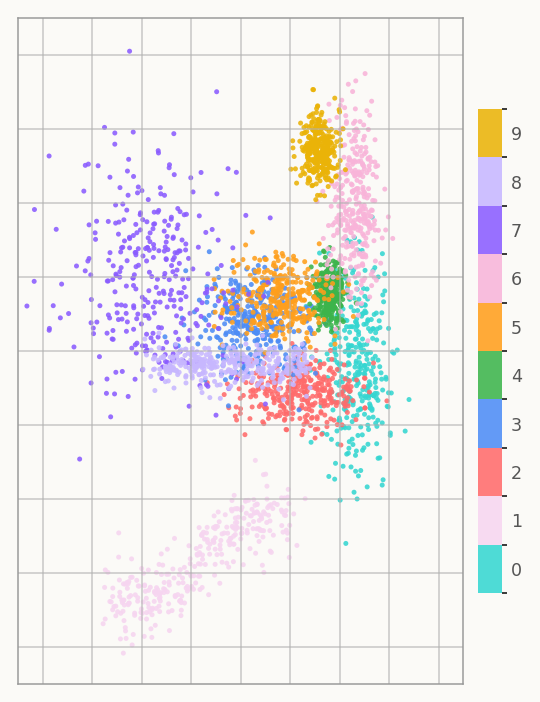
\includegraphics[width=3.8cm]{recon_only_space.png}};

  % explanation box
  \LatentNoteBox{1.00}{2.55}

  \node[
    anchor=west,
    text width=13.15cm,
    align=left,
    font=\footnotesize,
    text=ink
  ] at (1.35,1.82) {
    \textbf{Problem:} With only \textbf{reconstruction loss}, the model may reconstruct data well,
    but the latent space can become \textbf{irregular, discontinuous, and hard to sample from}.
    Random points may fall into weak regions, so generation becomes unreliable.
  };

\end{canvas}
\end{frame}

% ================================================================
% KULLBACK-LEIBLER (KL) DIVERGENCE
% ================================================================

\begin{frame}{Kullback-Leibler (KL) Divergence}

\begin{canvas}

% ================================================================
% OVERLAY 1 — WHAT KL DIVERGENCE MEASURES
% ================================================================

\fill[
    navy!7,
    rounded corners=5pt
]
(1.05,5.75) rectangle (14.95,7.05);

\draw[
    navy,
    line width=1.25pt,
    rounded corners=5pt
]
(1.05,5.75) rectangle (14.95,7.05);

\node[
    anchor=west,
    text width=12.9cm,
    align=left,
    font=\normalsize,
    text=ink
]
at (1.55,6.40)
{
    Measures the divergence between
    $q_{\phi}(z|x)$ and the prior $p(z)$,
    typically $\mathcal{N}(0,I)$.
};


% ================================================================
% OVERLAY 2 — REGULARIZATION PURPOSE
% ================================================================

\only<2->{

    \fill[
        navy!7,
        rounded corners=5pt
    ]
    (1.05,3.25) rectangle (14.95,5.35);

    \draw[
        navy,
        line width=1.25pt,
        rounded corners=5pt
    ]
    (1.05,3.25) rectangle (14.95,5.35);

    \node[
        anchor=west,
        text width=12.9cm,
        align=left,
        font=\normalsize,
        text=ink
    ]
    at (1.55,4.95)
    {
        \textbf{Regularization Purpose}
    };

    \node[
        anchor=west,
        text width=12.9cm,
        align=left,
        font=\normalsize,
        text=ink
    ]
    at (1.55,4.45)
    {
        Promotes a smooth, continuous latent space, fostering:
    };

    \fill[navy]
        (1.95,3.82) circle (2.1pt);

    \node[
        anchor=west,
        font=\normalsize\bfseries,
        text=ink
    ]
    at (2.25,3.95)
    {
        Continuity
    };

    \fill[navy]
        (1.95,3.5) circle (2.1pt);

    \node[
        anchor=west,
        font=\normalsize\bfseries,
        text=ink
    ]
    at (2.25,3.5)
    {
        Completeness
    };
}


% ================================================================
% OVERLAY 3 — KL FORMULA
% ================================================================

\only<3->{

    \fill[
        navy!7,
        rounded corners=5pt
    ]
    (1.05,0.95) rectangle (14.95,2.90);

    \draw[
        navy,
        line width=1.25pt,
        rounded corners=5pt
    ]
    (1.05,0.95) rectangle (14.95,2.90);

    \node[
        anchor=west,
        text width=12.9cm,
        align=left,
        font=\normalsize,
        text=ink
    ]
    at (1.55,2.45)
    {
        \textbf{KL Divergence Formula}
    };

    \node[
        text=navy,
        font=\Large
    ]
    at (8.00,1.65)
    {
        $\displaystyle
        \mathcal{L}_{KL}
        =
        D_{KL}
        \left(
        q_{\phi}(z|x)
        \,\|\, p(z)
        \right)
        =
        \int
        q_{\phi}(z|x)
        \log
        \frac{q_{\phi}(z|x)}
             {p(z)}
        \, dz
        $
    };
}

\end{canvas}

\end{frame}


% ================================================================
% EVIDENCE LOWER BOUND (ELBO)
% ================================================================

\begin{frame}{Evidence Lower Bound (ELBO)}

\begin{canvas}

% ================================================================
% OVERLAY 1 — ELBO OVERVIEW
% ================================================================

\fill[
    navy!7,
    rounded corners=5pt
]
(1.05,4.95) rectangle (14.95,6.65);

\draw[
    navy,
    line width=1.25pt,
    rounded corners=5pt
]
(1.05,4.95) rectangle (14.95,6.65);

\node[
    anchor=west,
    text width=12.9cm,
    align=left,
    font=\normalsize\bfseries,
    text=navy
]
at (1.55,6.28)
{
    ELBO: Overview
};

\node[
    anchor=west,
    text width=12.9cm,
    align=left,
    font=\normalsize,
    text=ink
]
at (1.55,5.65)
{
    ELBO balances two objectives:
    \textbf{Reconstruction Quality}
    and
    \textbf{Latent Space Regularization}.
};


% ================================================================
% OVERLAY 2 — GOAL / LOSS
% ================================================================

\only<2->{

    \fill[
        navy!7,
        rounded corners=5pt
    ]
    (1.05,2.00) rectangle (14.95,4.35);

    \draw[
        navy,
        line width=1.25pt,
        rounded corners=5pt
    ]
    (1.05,2.00) rectangle (14.95,4.35);

    \node[
        anchor=west,
        text width=12.9cm,
        align=left,
        font=\normalsize\bfseries,
        text=navy
    ]
    at (1.55,3.96)
    {
        Goal
    };

    \node[
        anchor=west,
        text width=12.9cm,
        align=left,
        font=\normalsize,
        text=ink
    ]
    at (1.55,3.43)
    {
        Maximizing ELBO is equivalent to minimizing the VAE loss:
    };

    \node[
        text=navy,
        font=\Large
    ]
    at (8.00,2.75)
    {
        $\displaystyle
        \mathcal{L}_{\mathrm{VAE}}
        =
        \mathcal{L}_{\mathrm{recon}}
        +
        \mathcal{L}_{\mathrm{KL}}
        $
    };

    
}

\end{canvas}

\end{frame}
\begin{frame}{ELBO : Impact Visualization}
\begin{canvas}

% =========================================================
% HEADINGS
% =========================================================

\node[
  font=\small\bfseries,
  text=ink,
  align=center
] at (3.15,7.4)
{Only reconstruction loss};

\node[
  font=\small\bfseries,
  text=ink,
  align=center
] at (8.00,7.4)
{Only KL divergence};

\node[
  font=\small\bfseries,
  text=ink,
  align=center
] at (12.85,7.4)
{Reconstruction loss\\and KL divergence};


% =========================================================
% IMAGES
% =========================================================

\node at (3.15,4.75)
{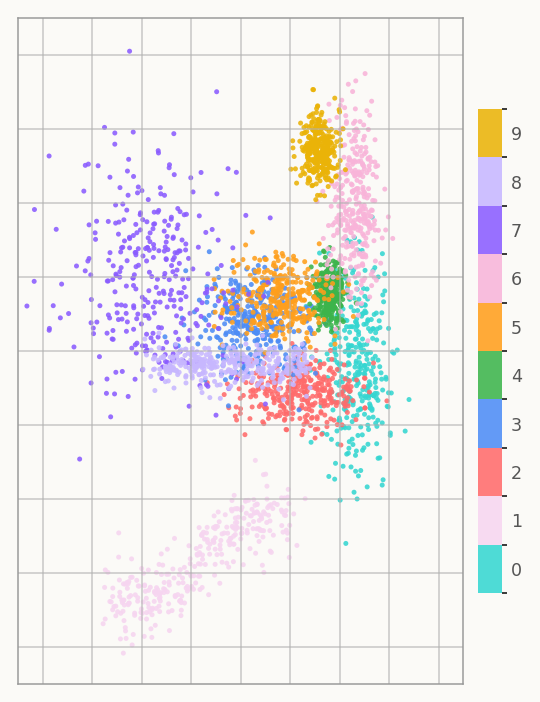
\includegraphics[width=3.2cm]{recon_only_space.png}};

\node at (8.00,4.75)
{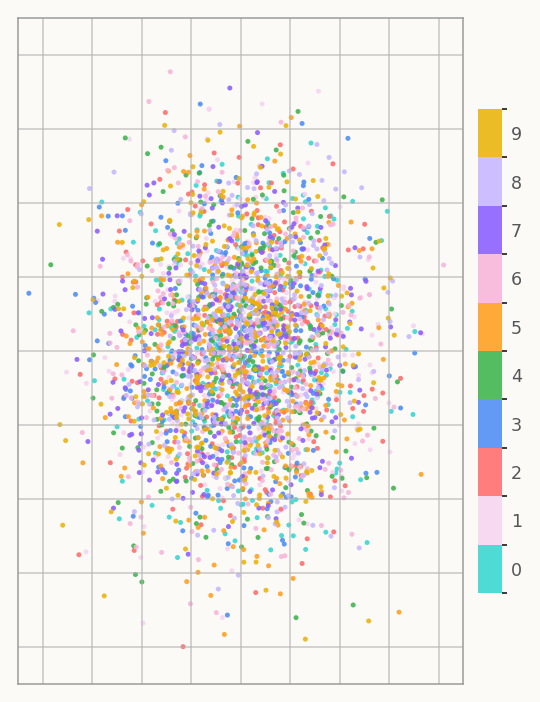
\includegraphics[width=3.2cm]{kl_only_space.png}};

\node at (12.85,4.75)
{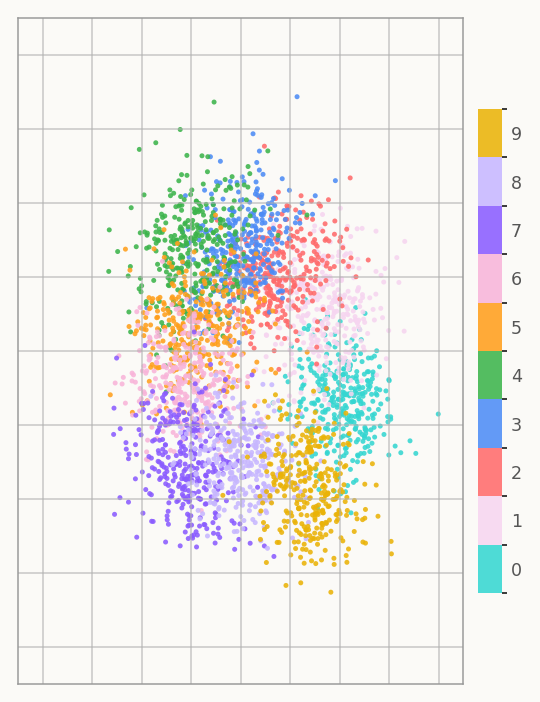
\includegraphics[width=3.2cm]{recon_kl_space.png}};


% =========================================================
% ELBO DIALOG BOX
% =========================================================

\fill[
  navy!7,
  rounded corners=5pt
]
(0.85,0.95) rectangle (15.15,2.45);

\draw[
  navy,
  line width=1.25pt,
  rounded corners=5pt
]
(0.85,0.95) rectangle (15.15,2.45);


\node[
  anchor=west,
  text width=13.3cm,
  align=left,
  font=\footnotesize,
  text=ink
] at (1.25,1.75)
{
  \textbf{ELBO combines both goals:}\quad
  $\displaystyle
  \mathrm{ELBO}
  =
  \mathbb{E}_{q_\phi(z\mid x)}
  \!\left[\log p_\theta(x\mid z)\right]
  -
  D_{KL}\!\left(
  q_\phi(z\mid x)\,\|\,p(z)
  \right)
  $
  \\[5pt]
  In practice:
  \textbf{reconstruct well}
  and
  \textbf{keep the latent space regular}.
};

\end{canvas}
\end{frame}

\end{document}
